% Juneki Hong and Michael Tango
% Declarative Methods
% Professor Eisner
% May 3, 2013


\documentclass{article}
\usepackage{acl2012}
\usepackage{times}
\usepackage{latexsym}
\usepackage{amsmath}
\usepackage{multirow}
\usepackage{url}
\usepackage{tikz}

\usepackage[english]{babel}
\usepackage{graphicx}
\setlength\titlebox{6.5cm}    % Expanding the titlebox


\title{Declarative Methods Term Project: \\ JumanG}
\author{Juneki Hong and Michael Tango}

%\usepackage[ampersand]{easylist}

\date{}
\begin{document}
\maketitle

\begin{abstract}
In this paper we introduce JumanG, a system that will attempt to display graphs in an effective or aesthetically pleasing way. We implement several types of familiar graph layout methods, and then given a graph we perform some analysis to attempt to decide which method to perform. We will compare the results of our implemented graph layout methods to the results of similar GraphViz layout programs, and we will show how our display decision process automatically handles a variety of graphs appropriately.
\end{abstract}

\section{Introduction}
Graphs can represent a wide range of data and information, and the task of visualizing graphs is important in revealing the patterns and underlying structure within them. Although many heuristics are available for what determines a "good" visualization such as number of edge crossings, regular spacing, and node overlaps, in the end the best way to visualize a given graph might be circumstantial or domain specific. 
There are subsequently several specialized layout methods that can perform well in particular instances for effective or aesthetic display.
 
Programs such as GraphViz have several different layout methods, but this relies on the user to decide which one to use. 
In other words, the user is required to have an intuition about how each solver works and would make their graph appropriately look the best. Instead of having the user say \textit{how} the graph should be displayed, we intend to let the user express only that a graph should be displayed.

JumanG seeks to determine which layout method is most appropriate by doing some analysis on some features of the graph such as its size, directedness, branching factor, and cyclicity.

\section{The JumanG Pipeline}
The JumanG system has three main sections in its pipeline. It has an \textit{encoder} that parses in a graph specification into its internal data structures, a set of \textit{solvers} that will lay out the graph and assign coordinate values to display, and a \textit{decoder} that takes the processed graph and outputs out to Tikz LaTeX where it can be displayed on the screen.

\subsection{The Encoder and the Dot Language}
The encoder for JumanG starts by reading in a Dot file. 
Dot is a Little Language used for the specification of graphs, and so we wanted to use Dot files as a graph description for which we could parse in and process.
We built a parser that accomplishes this, passing off the internal graph to our solvers.


\subsection{Analysis and Solvers}
We implemented several different graph layout solvers (as well as call one from GraphViz). These solvers all implement previous well known layout methods. They work well in different situations, and JumanG attempts to decide which of these would be the best to use.

In order to do this, JumanG decides based on the features extracted. Directed acyclic graphs would be run with the Layered Solver, directed and undirected graphs with very high branching factor would be run with our Radial Solver, directed rings would be run with the GraphViz Circo Solver, and all other undirected graphs and graph meshes would be run with our Springs Solver. 

In this way, we formed a Decision Tree that would allow JumanG's analysis to determine which solver to run the given graph against.


\subsection{Radial Solver}
Radial displays have been used to display trees in a way different from a typical top-down approach.
Introduced in 1992 by Eades (EADES CITATION), this layout places the branches circularly around the root outwards, drawing 
nodes at different radii from the center. We implemented our own Radial solver that uses similar techniques to the original
method. We wrote our solver to evenly distribute nodes around the root at each level, rather than the typical style of weighting 
the nodes based on the subnodes. We also chose to display nodes at their closest level to root. 
This allows the solver to draw non-tree graphs fairly well. Here is our solver against Graphviz's twopi on some of the same graphs: 
%TODO (INSERT COMPARISON GRAPHS) 

A radial solver can be used rather than a standard layered solver for drawing graphs that are much wider than they are deep. Our metric 
for determining whether the radial solver should be used is given by a measure of width: 
$$width = \frac{|nodes|}{depth_{graph}}$$

Here are some results based on our radial solver:
%TODO add more metanalysis here) (Insert some results here)





\begin{figure}
\caption{Radial Solver on a graph with high branching factor}
\begin{tikzpicture}[scale=0.40, transform shape]
	\tikzstyle{every node} = [circle, fill=gray!30, minimum size = 1.4cm]
	\node (24) at (3.52, 8.28) {24};
	\node (25) at (1.25, 8.91) {25};
	\node (26) at (-8.34, -3.37) {26};
	\node (27) at (-7.55, -4.90) {27};
	\node (20) at (1.55, -5.80) {20};
	\node (21) at (3.86, -4.60) {21};
	\node (22) at (5.20, -3.00) {22};
	\node (23) at (5.91, -1.04) {23};
	\node (28) at (-6.89, -5.79) {28};
	\node (29) at (7.19, -5.42) {29};
	\node (1) at (0.00, 0.00) {1};
	\node (3) at (0.00, 3.00) {3};
	\node (2) at (2.60, 1.50) {2};
	\node (5) at (-2.60, -1.50) {5};
	\node (4) at (-2.60, 1.50) {4};
	\node (7) at (2.60, -1.50) {7};
	\node (6) at (0.00, -3.00) {6};
	\node (9) at (5.56, 2.25) {9};
	\node (8) at (5.96, 0.73) {8};
	\node (11) at (3.69, 4.73) {11};
	\node (10) at (4.79, 3.61) {10};
	\node (13) at (-1.55, 5.80) {13};
	\node (12) at (1.55, 5.80) {12};
	\node (15) at (-5.96, -0.73) {15};
	\node (14) at (-5.20, 3.00) {14};
	\node (17) at (-4.79, -3.61) {17};
	\node (16) at (-5.56, -2.25) {16};
	\node (19) at (-1.55, -5.80) {19};
	\node (32) at (8.86, -1.56) {32};
	\node (31) at (8.16, -3.80) {31};
	\node (30) at (7.71, -4.64) {30};
	\node (18) at (-3.69, -4.73) {18};
	\draw [->] (22)--(29);
	\draw [->] (22)--(30);
	\draw [->] (22)--(31);
	\draw [->] (23)--(32);
	\draw [->] (1)--(2);
	\draw [->] (1)--(3);
	\draw [->] (1)--(4);
	\draw [->] (1)--(5);
	\draw [->] (1)--(6);
	\draw [->] (1)--(7);
	\draw [->] (3)--(12);
	\draw [->] (3)--(13);
	\draw [->] (2)--(8);
	\draw [->] (2)--(9);
	\draw [->] (2)--(10);
	\draw [->] (2)--(11);
	\draw [->] (5)--(15);
	\draw [->] (5)--(16);
	\draw [->] (5)--(17);
	\draw [->] (5)--(18);
	\draw [->] (4)--(14);
	\draw [->] (7)--(21);
	\draw [->] (7)--(22);
	\draw [->] (7)--(23);
	\draw [->] (6)--(19);
	\draw [->] (6)--(20);
	\draw [->] (12)--(24);
	\draw [->] (12)--(25);
	\draw [->] (17)--(27);
	\draw [->] (17)--(28);
	\draw [->] (16)--(26);
\end{tikzpicture}
\end{figure}








\subsection{Springs solver}

The Springs algorithm, as outlined by Kawai and Kamada\cite{springs}, computes a layout for a graph by running a physics simulation on the graph. All of the nodes are set to repel each other, while the edges are set as ``springs" to hold the nodes together. Our solver scales the repelling forces of the nodes based on how densely connected the graphs are, in order to prevent nodes being spaced too close or far apart in the end.

This was the repulsion force used in our Springs solver:
$$ f_r = \frac{|edges|}{|nodes|}^3 \frac{1}{d^2} $$
Where d is the euclidean distance between any two nodes. 

We defined the attraction function between two connected nodes as a linear factor of the distance between two nodes. With the constraints in place the simulation attempts to minimize the total energy in the graph.

\subsubsection{Springs solver's Initialization}
The Springs solver also requires the nodes to have an initial configuration. 
%TODO citation of book
suggests two possible approaches. The first being random placement, where all of the nodes are randomized, and the second being based on geodesic distance. We have implemented both options, the second option using the Radial solver as an alternative to this geodesic distance initialization. 

The Radial initialization works well for graphs with sparse connections, spreading the nodes out, and giving the Springs algorithm a good starting point to begin minimizing the energy in the system. More densly connected graphs do not work as well using this, and so we default back to random jitter perturbation initialization.

We measured connectivity as:
$$connectivity = \frac{|nodes|}{|edges|}$$
And based on some empirical testing we determined to use randomized initialization on graphs with connectivity higher than 3.


\begin{figure}
\caption{A Sparsely Connected Graph with the Springs Solver with Radial Initialization}
\begin{tikzpicture}[scale=0.40, transform shape]
	\tikzstyle{every node} = [circle, fill=gray!30, minimum size = 1.8cm]
	\node (H4) at (0.16, -4.08) {H4};
	\node (H5) at (-5.44, -2.10) {H5};
	\node (H2) at (3.43, 8.65) {H2};
	\node (H3) at (-4.62, 3.79) {H3};
	\node (H0) at (8.17, 0.76) {H0};
	\node (H1) at (9.03, 6.64) {H1};
	\node (C1) at (-1.14, 0.52) {C1};
	\node (C0) at (4.71, 4.05) {C0};
	\draw [-] (H4)--(C1);
	\draw [-] (H5)--(C1);
	\draw [-] (H2)--(C0);
	\draw [-] (H3)--(C1);
	\draw [-] (H0)--(C0);
	\draw [-] (H1)--(C0);
	\draw [-] (C1)--(C0);
	\draw [-] (C1)--(H3);
	\draw [-] (C1)--(H4);
	\draw [-] (C1)--(H5);
	\draw [-] (C0)--(H0);
	\draw [-] (C0)--(H1);
	\draw [-] (C0)--(H2);
	\draw [-] (C0)--(C1);
\end{tikzpicture}
\end{figure}



\begin{figure}
\caption{A Densely Connected Graph with the Springs Solver with Random Jitter Initialization}
\begin{tikzpicture}[scale=0.50, transform shape]
	\tikzstyle{every node} = [circle, fill=gray!30, minimum size = 1.8cm]
	\node (k3) at (0.72, 3.87) {k3};
	\node (k2) at (-3.06, -2.52) {k2};
	\node (k1) at (1.41, -3.52) {k1};
	\node (k5) at (-3.49, 2.05) {k5};
	\node (k4) at (3.75, 0.43) {k4};
	\draw [-] (k3)--(k1);
	\draw [-] (k3)--(k2);
	\draw [-] (k3)--(k4);
	\draw [-] (k3)--(k5);
	\draw [-] (k2)--(k1);
	\draw [-] (k2)--(k3);
	\draw [-] (k2)--(k4);
	\draw [-] (k2)--(k5);
	\draw [-] (k1)--(k2);
	\draw [-] (k1)--(k3);
	\draw [-] (k1)--(k4);
	\draw [-] (k1)--(k5);
	\draw [-] (k5)--(k1);
	\draw [-] (k5)--(k2);
	\draw [-] (k5)--(k3);
	\draw [-] (k5)--(k4);
	\draw [-] (k4)--(k1);
	\draw [-] (k4)--(k2);
	\draw [-] (k4)--(k3);
	\draw [-] (k4)--(k5);
\end{tikzpicture}
\end{figure}


\subsection{Layered Solver}
Layered graph drawing is an approach to arranging directed acyclic graphs.


\subsection{Circo Solver}
Circo is a graph layout solver available from within GraphViz that specializes in arranging circular graphs. 
We use Circo as one of our available graph solvers because we did not implement our own version of a circular layout solver.

%TODO put in an example picture
\begin{figure}[h!]
\caption{A Ring Graph solved by the Circo Solver}
\centering
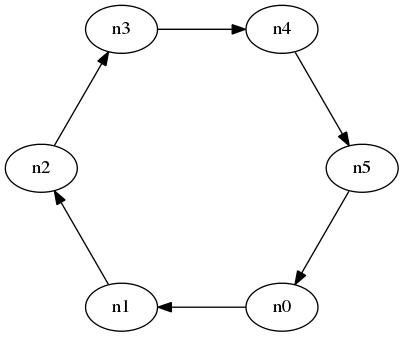
\includegraphics[width=0.3\textwidth]{circo.jpg}
\end{figure}

In our analysis of the given graph, we can determine that a graph is a directed cycle if there are no root nodes, that is nodes that do not have inward edges pointing to them. When a graph is a directed cycle, the Circo Solver tends to have good results. Our Springs Solver does a good job with undirected cycles because the edges ``pull" in both directions, and the balanced forces can properly work on the simulation. 

\begin{figure}
\caption{The same Undirected Ring Graph solved by the Springs Solver}
\begin{tikzpicture}[scale=0.40, transform shape]
	\tikzstyle{every node} = [circle, fill=gray!30, minimum size = 1.8cm]
	\node (n0) at (-0.17, -0.79) {n0};
	\node (n1) at (-0.17, 4.10) {n1};
	\node (n2) at (4.06, 6.54) {n2};
	\node (n3) at (8.30, 4.09) {n3};
	\node (n4) at (8.30, -0.80) {n4};
	\node (n5) at (4.06, -3.24) {n5};
	\draw [-] (n0)--(n1);
	\draw [-] (n0)--(n5);
	\draw [-] (n1)--(n0);
	\draw [-] (n1)--(n2);
	\draw [-] (n2)--(n1);
	\draw [-] (n2)--(n3);
	\draw [-] (n3)--(n2);
	\draw [-] (n3)--(n4);
	\draw [-] (n4)--(n3);
	\draw [-] (n4)--(n5);
	\draw [-] (n5)--(n4);
	\draw [-] (n5)--(n0);
\end{tikzpicture}
\end{figure}


\subsection{The Decoder}
We decided to output our graphs to TikZ syntax, a package for drawing graphs in LaTeX, which we felt was a very appropriate format, and allowed us to ignore the 
the difficulties of rendering graphics. This also allows us to directly embed our graphs into other LaTeX documents, such as this one. The algorithm for 
writing the graphs is not particularly clever or efficient, and currently we have only one format, but the TikZ package is featureful enough that adding arbitrary
features to the display would not be hard.


\section{Experimental Comparison}


\section{Future Work}


\section{Conclusions}

\bibliographystyle{plain}
\bibliography{citations}




\end{document}
